{ %define guard

\delimitershortfall=-0.10pt

%region settings
\newcommand{\given}{\,\middle|\,}               % conditional probability

\newcommand{\Reals}{\mathds{R}}                 % Reals set

\newcommand{\defeq}{\vcentcolon=}               % definition
\newcommand{\eqdef}{=\vcentcolon}               % reverse definition

\renewcommand{\l}{\mathopen{}\left}             % \left alias
\renewcommand{\r}{\vphantom{1j}\right}          % \right alias

\renewcommand{\P}{\mathrm{P}}                   % probability
\newcommand{\E}{\mathrm{E}}                     % expected value
\newcommand{\e}{\mathrm{e}}                     % euler number
\newcommand{\nf}{\nicefrac}                     % nicefrac
\renewcommand{\d}{\cdot}                        % multiplication
%endregion

\cleardoublepage
\section{Aula 17 de Outubro de 2019}
\label{2019_10_17}

% #region continuação teo5 caso ->infty
\subsection*{\it Continuação}

\begin{teorema}
  \normalfont\textbf{[T5.]}
  Seja
  \vspace*{-\baselineskip}
  \[
    p = \nicefrac{1}{n}\l(\log n + c_n\r)
  \]
  então
  \vspace*{-\baselineskip}
  \[
    \lim_{n\rightarrow\infty} \P\l(G\l(n,\ p\r) \text{ é conexo}\r) = \l\{\begin{array}{ll}
      0                               & \text{se } c_n\rightarrow-\infty                            \\
      \mathrel{e}^{-\mathrel{e}^{-c}} & \text{se } c_n\rightarrow c\in\Reals                        \\
      1                               & \text{se } c_n\rightarrow\infty                             \\
    \end{array}\r.
  \]
\end{teorema}

Seja $X_k=\#$componentes de $G\l(n,\ p\r)$ com $k$ vértices.

Por exemplo, $X_1=\#$vértices isolados.

\begin{proof}[Prova caso $c_n\rightarrow\infty$]
  $ $\newline
  Temos
  \vspace*{-\baselineskip}
  \begin{align*}
    \P\l(G\l(n,\ p\r)\text{ é desconexo}\r)
      &=    \P\l(\sum_{1\leq k\leq\nf{n}{2}}X_k\geq 1\r)
      \leq  \E\l(\sum_{1\leq k\leq\nf{n}{2}}\r)                                                     \\
      &=    \sum_{1\leq k\leq\nf{n}{2}}\E\l(X_k\r)
      \leq  \sum_{1\leq k\leq\nf{n}{2}}\binom{n}{k}\l(1-p\r)^{k\l(n-k\r)}
  \end{align*}

  Também temos
  \begin{align*}
    \sum_{1\leq k\leq n^{\nf{3}{4}}}\binom{n}{k}\l(1-p\r)^{k\l(n-k\r)}
      &\leq \sum_{1\leq k\leq n^{\nf{3}{4}}}\l(\nf{\e n}{k}\d\e^{-p\l(n-k\r)}\r)^k                  \\
      &\leq \sum_{1\leq k\leq n^{\nf{3}{4}}}
              \l(\nf{\e n}{k}\d\e^{-\log n-c_n+\smash{\overbrace{2\nf{k}{n}\log n}^{o(1)}}}\r)^k    \\
      &\leq \sum_{1\leq k\leq n^{\nf{3}{4}}}\l(\nf{2}{k}\d\e^{1-c_n}\r)^k
      \leq  3\e^{1-c_n} 
      \rightarrow 0
  \end{align*}

  Ademais,
  \begin{align*}
    \sum_{n^{\nf{3}{4}}<k\leq\nf{n}{2}}\binom{n}{k}\l(1-p\r)^{k\l(n-k\r)}
      &\leq \sum_{n^{\nf{3}{4}}<k\leq\nf{n}{2}}
              \l(\e\d\smash{\overbrace{\nf{n}{k}}^{<n^{\nf{1}{4}}}}\d
              \e^{\smash{\overbrace{-p\l(n-k\r)}^{\geq\nf{n}{2}}}}\r)^k                             \\
      &\leq \sum_{n^{\nf{3}{4}}<k\leq\nf{n}{2}}\l(\e\d n^{\nf{1}{4}}\d\e^{\nf{-\log n}{2}}\r)^k
      \leq  n^{\nf{1}{5}\d n^{\nf{3}{4}}}
      \rightarrow 0
  \end{align*}
\end{proof}
% #endregion

% #region comentários sobre teo5 caso ->c
\clearpage
\subsection*{\normalfont Comentários sobre o caso $c_n\rightarrow c\in\Reals$.}$ $\newline

Podemos usar
\vspace*{-\baselineskip}
\[
  \E\l(X_k\r) = \binom{n}{k} \l(1-p\r)^{k\l(n-k\r)} k^{k-2} p^{k-1}
\]

Pelo Teorema de Cayley [<\href{https://en.wikipedia.org/wiki/Cayley%27s_formula}{https://en.wikipedia.org/wiki/Cayley\%27s\_formula}>: \#árvores geradoras de ordem $n$, temos que
\[
  k^{k-2} p^{k-1} = p\l(k\,p\r)^{k-2} \rightarrow 0 \text{ se } k>2
\]

Segue que no outro caso caso $c_n\rightarrow c$
\[
  \P\l(\sum_{k=2}^{\nf{n}{2}} X_k \geq 1\r) = \E\l(\sum_{k=2}^{\nf{n}{2}} X_k\r) \rightarrow 0
\]

Concluímos que, com prob. $\rightarrow1$, $G\l(n,\ p\r)$ é composto por uma componente e $X_1$ vértices isolados.

Assim, $G\l(n,\ p\r)$ é conexo se e só se $X_1=0$.

Vale que $X_1$ converge em probabilidade para uma v.a. $\mathrm{Pois}\l(\e^{-c}\r)$.

Distribuição \textbf{Poison} [<\href{https://en.wikipedia.org/wiki/Poisson_distribution}{https://en.wikipedia.org/wiki/Poisson\_distribution}>]:
\begin{itemize}
  \item $Z\sim\mathrm{Pois}\l(\lambda\r)$;
  \item $Z\in\mathbb{N}$;
  \item $\P\l(Z=t\r) = \e^{-\lambda}\d\nf{\lambda^t}{t!}$, $t>0$;
  \item $\E\l(Z\r) = \lambda$; e 
  \item $\P\l(Z=0\r) = \e^{-c}$.
\end{itemize}

Lembrando que $\E\l(X_1\r)\rightarrow\e^{-c}$:
\[
  \lim_{n\rightarrow\infty} \P\l(X_1=t\r)
    = \P\l(\mathrm{Pois}\l(\e^{-c}\r)=t\r)
    = \e^{-\e^{-c}}\,\nf{\l(\e^{-c}\r)^t}{t!}
\]

Para todo $t$ fixo. Em particular,
\[
  \P\l(G\l(n,\ p\r) \text{ é conexo}\r) = \lim_{n\rightarrow\infty} \P\l(X_1=0\r)=\e^{-\e^{-c}}
\]
%endregion

% #region teoB-Th87
\clearpage
\subsection{Teorema de Bollubón e Thomson}$ $\newline

[\textit{Primeiro teorema para qualquer propriedade crescente. Antes, era preciso provar para cada uma.}]

[\textit{Prova original era com teoria dos conjuntos, mais complicada.}]

\begin{teorema}
  \normalfont\textbf{[T6 B-Th'87.]}
  Seja $\mathcal{P}$ uma propriedade não trivial crescente. Então $\mathcal{P}$ admite uma função limiar:
  \vspace*{-\baselineskip}
  \begin{align*}
    \P\l(G_p\in\mathcal{P}\r)
      &\rightarrow \l\{\begin{array}{ll}
                      0 & \text{se } p \ll p_0  \\
                      1 & \text{se } p \gg p_0  \\
                    \end{array}\r.                                                                  \\
    \P\l(G_p\not\in\mathcal{P}\r)
      &\leq\epsilon
  \end{align*}
\end{teorema}

\begin{proof}[(Esboço)]$ $\newline
  Seja $p_0<p_0\l(n\r)$ tal que
  \vspace*{-\baselineskip}
  \[
    \P\l(G\l(n,\ p\r)\in\mathcal{P} = \nf{1}{2}\r)
  \]

  Fixe $\epsilon>0$, e seja $t$ t.q. $\l(\nf{1}{2}\r)t\leq\epsilon$. Considere $t$ cópias independentes de $G\l(n,\ p\r)$, digamos $G_1,\ \ldots,\ G_t$. Seja $p'$ t.q. $1-p'=(1-p_0)^t$. Temos
  \[
    G\l(n,\ p'\r) = G_1\cup\ldots\cup G_t
  \]

  Temos que
  \vspace*{-\baselineskip}
  \[
    \P\l(G\l(n,\ p\r)\not\in\mathcal{P}\r)
      \leq \prod_{1\leq i\leq t} \P\l(G_i\not\in\mathcal{P}\r)
      = \l(\nf{1}{2}\r)^t
      \leq \epsilon
  \]

  Segue que se $p\gg p_0$, então
  \[
    \P\l(G\l(n, p\r)\not\in\mathcal{P}\r) \rightarrow 0
  \]

  Um argumento análogo prova que se $p\ll p_0$, então
  \[
    \P\l(G\l(n, p\r)\in\mathcal{P}\r) \rightarrow 0
  \]
\end{proof}
% #endregion

% #region transição de fase em GNP
\clearpage
\subsection{Transição de fase em $G(n,\ p)$}$ $\newline

[$G_t\approx G\l(n,\ \nf{t}{\binom{n}{2}}\r)$, $t=p\binom{n}{2}\sim p\,\nf{n^2}{2}$, $p=\nf{1}{n}$.]

[Propriedades crescente têm uma transição tipo $\l[a\,p,\ b\,p\r]$, com $a\rightarrow0$ e $b\rightarrow\infty$.]

Seja $L_k\l(G\r)=$\#vértices da $k$-ésima maior componente de $G$. Claro que $L_1\l(G\r)\geq L_1\l(G\r)\geq\ldots$.

\begin{teorema}
  \normalfont\textbf{[T7.]}
  Seja $\epsilon>0$ uma constante fixa.
  \begin{enumerate}
    \item Se $p=\nf{\l(1-\epsilon\r)}{n}$, então q.c. $G\l(n,\ p\r)$ é t.q. $L_1\l(G\l(n,\ p\r)\r)\leq c\,\log n$, onde $c=c_\epsilon$.
    \item Se $p=\nf{\l(1+\epsilon\r)}{n}$, então q.c. $G\l(n,\ p\r)$ é t.q. $L_1\l(G\l(n,\ p\r)\r)\geq c\,n$ e $L_2\l(G\l(n,\ p\r)\r)\leq c\,\log n$, onde $c=c_\epsilon$.
  \end{enumerate}
\end{teorema}

\begin{proof}[Prova]$ $\newline
  Vamos provar que se $p=\nf{\l(1+\epsilon\r)}{n}$, então $L_1\l(G\l(n,\ p\r)\r)\geq\nf{1}{24}\,\epsilon^2\,n$ com prob. $\rightarrow1$.

  Usamos busca em profundidade:
  \begin{enumerate}
    \item $U\leftarrow V=V\l(G\r)$;
    \item $G=G\l(n,\ p\r)$;
    \item $E\leftarrow\varnothing$;
    \item $F\leftarrow\varnothing$; e
    \item Para cada $v\in V$, se $v\in U$ então $\texttt{dfs}\l(v\r)$.
  \end{enumerate}
\end{proof}

\begin{itemize}[label={}]
  \item $\texttt{dfs}\l(v\r)$
  \begin{itemize}[label={}]
    \item $F\leftarrow F\cup\l\{v\r\}$
    \item $U\leftarrow U\setminus\l\{v\r\}$
    \item Para cada $w\neq v$
    \begin{itemize}[label={}]
      \item se $w\in U$
      \item então se $\l\{v,\ w\r\}\in\E\l(G\l(n,\ p\r)\r)$ (query)
      \begin{itemize}[label={}]
        \item $\texttt{dfs}\l(w\r)$
      \end{itemize}
    \end{itemize}
    \item $E\leftarrow E\cup\l\{v\r\}$
    \item $F\leftarrow F\setminus\l\{v\r\}$
  \end{itemize}
\end{itemize}

Executamos a $\texttt{dfs}$ até fazermos $t=\delta\,n^2$ queries, onde $\delta=\nf{\epsilon}{4}$.

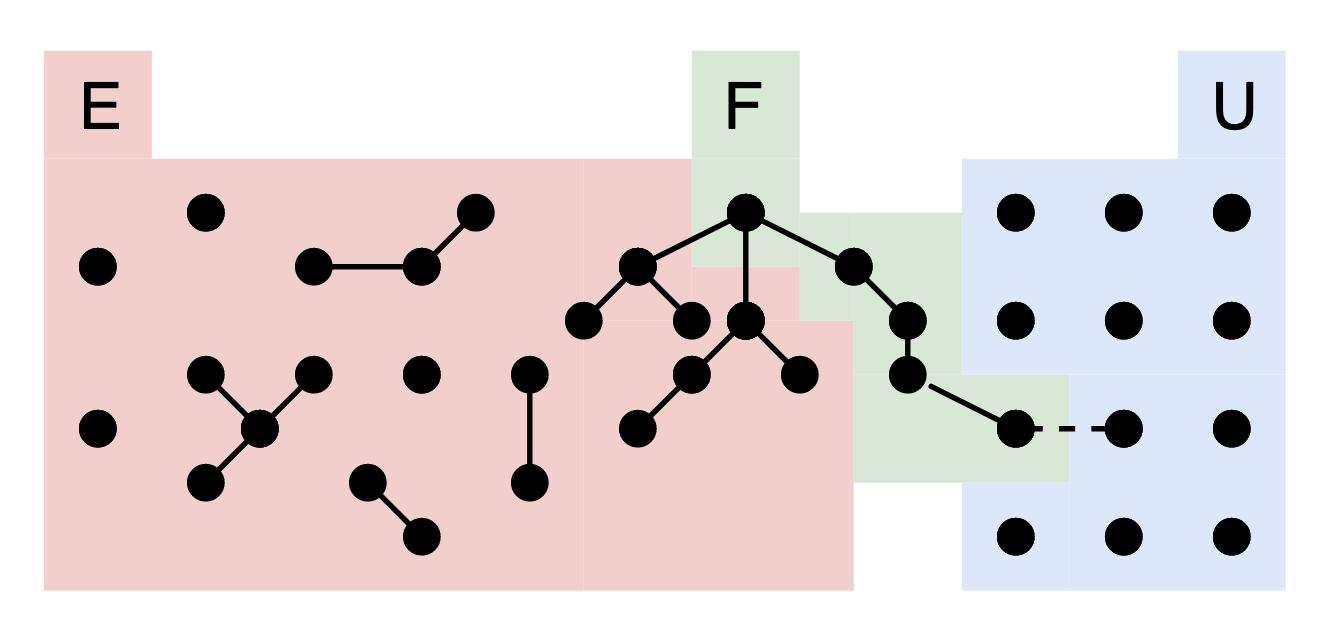
\includegraphics[width=0.75\textwidth]{aulas/10_17/dfs.png}

\begin{observacao}
  O valor esperado de queries com resposta positiva é $\delta\,n^2\,p=\delta\l(1+\epsilon\r)$. Com prob. $\rightarrow1$, temos que o número de respostas positivas é t.q.
  \[
    \delta\l(1+\nf{\epsilon}{2}\r)n \leq s \leq \delta\l(1+2\,\epsilon\r)n
  \]
  
  Por Chebyshev ou Chernoff.
  
  Sem perda de generalidade, $\epsilon\leq\nf{1}{4}$.
\end{observacao}

\begin{fato}
  \normalfont
  $\not\exists$ arestas  em $G\l(n,\ p\r)$ entre $E$ e $U$.
\end{fato}

Provamos que, se $L_1\l(G\l(n,\ p\r)\r)<\nf{1}{24}\,\epsilon^2\,n$, então $\l|E\r|\,\l|U\r|>t$.

Isso é uma contradição.

Vamos provar que, em algum momento, $\l|F\r|\geq\nf{1}{24}\,\epsilon^2\,n$, c.c. $\l|E\r|\,\l|U\r|>t$.
% #endregion

}
